\chapter{Customizing and debugging PM2}

\stamp $Id: customizing.tex,v 1.4 2001/04/18 15:13:12 bouge Exp $

\section{Introducing PM2 flavors}

You have now compiled and run a few PM2 programs. It is time to have a
look at the underlying machinery. The key feature is the notion of
\emph{flavor}, which we explain in detail below. Technically speaking,
a PM2 module is a library to be linked with your program. For
instance, module \|pm2| is library \|libpm2.a|. It is the job of the
\|pm2-config| utility to automagically generate the right compiling
and linking set of directives for the various libraries.
\begin{shell}
# Assuming you use csh...
setenv CC       "`pm2-config --cc`"
setenv CFLAGS   "`pm2-config --cflags`"
setenv LIBS     "`pm2-config --libs`" 
$CC $CFLAGS hello.c $LIBS -o hello
\end{shell}

It is important to realize at this point that the various PM2 modules
are independently compiled into \emph{separate} libraries. Yet, these
libraries are \emph{strongly} dependent one on each other, and they
are moreover dependent on the directives used in compiling the main
program. Therefore, uttermost care is needed in managing the various
sets of compiling and linking directives, as they \emph{must} be
consistent. 

Another aspect is that many users are interested in using
\emph{several} versions of PM2 at a time. For instance, you may wish
to compare the performance of a given user program on a Myrinet and on
a SCI network within the same benchmarking session. Or, you may use a
version of the program compiled with all the debugging features turned
on, and another one aggressively optimized. You may even compare a
version of PM2 compiled with some C~compiler against another version
compiled with another one.  Such kind of decisions have a strong
influence on the resulting PM2 libraries. Changing the network from
Myrinet to SCI amounts to recompiling the Madeleine module.  Changing
the mode from debugging to optimizing actually results in recompiling
all the libraries from scratch. This is a not trivial operation, which
consumes time and resources.

\begin{note}
  LB to RN: Is the name of the C compiler included in the flavor?
\end{note}

These two motivations have led to the notion of \emph{PM2 flavors}. A PM2
flavor is simply a set of compiling and linking options for the user
program and the various modules of PM2: Marcel, Madeleine, and
various other ancillary modules. It is always assumed that the user
program and the modules have been compiled and linked with the
\emph{same} flavor. Unfortunately, there is no easy way to enforce
this in the C/Unix framework. The method used in PM2 to enforce global
consistency is following. 
\begin{itemize}
  
\item The list of all currently available flavors is provided by
  command \|pm2-flavor list|.

\item At any point, the currently active flavor is the value of shell
  variable \|PM2_FLAVOR|. Alternatively, most PM2 commands honor a
  \|--flavor=xxx| flag, so that you can easily manage several flavors
  at the same time within a makefile or a script. The default of
  \|xxx| is the value of variable \|PM2_FLAVOR|.
  
  \begin{warning}
    The \|PM2_FLAVOR| variable should most preferably be set to
    something! Remember to \|export| it if you use \|sh|-like
    shells.
  \end{warning}
  
\item Flavor \|xxx| is kept in file \|${PM2_HOME}/.pm2/flavors/xxx|, as
  provided by command \|pm2-flavor find --flavor=xxx|.
  \begin{warning}
    These files are automagically generated by the tools to be presented
    below. Do not edit by hand!
  \end{warning}
  
\item The list of options defined by flavor \|xxx| is provided by
  command \|pm2-flavor get --flavor=xxx|.

\item The internal consistency of flavor \|xxx| can be check by
  command  \|pm2-flavor check --flavor=xxx|. A flavor may be
  regenerated using command \|pm2-flavor regenerate --flavor=xxx|.

\item When a module is compiled with  flavor \|xxx|, then the
  resulting object code is placed into directory
  \|${PM2_BUILD_DIR}/xxx|. You may thus have several versions of PM2
  ready for use at the same time. 
  
\item To compile and link a user program with flavor \|xxx|, use the
  flags generated by commands \|pm2-config --cflags| and \|pm2-config
  --libs|, as exemplified in the Makefile on
  Figure~\ref{prog:Makefile1}.

\end{itemize}

\section{Making your own, personal PM2 flavors}

You know \emph{what} a flavor is, and more or less \emph{why} it is
so. Let us now learn \emph{how} they can be used. Assume for instance
that you have been using flavor \|pm2| since your (PM2-)birth:
\|setenv PM2_FLAVOR pm2|. After having grown up, you are now starting
feeling somehow unsatisfied with it, almost frustrated. No problem:
PM2 has something for you: \|ezflavor|! (To be pronounced:
\emph{ee-zee-flavor}.)

The \|ezflavor| utility is a graphic interface to list, modify, check,
regenerate flavors all in once. As it is highly dependent on the
operating system you are running, you first have to compile it:
\begin{shell}
ravel% cd ${PM2_ROOT}/ezflavor 
ravel% make 
\end{shell}
The binary will be installed in
\|${PM2_HOME}/.pm2/bin/ezflavor_AAA_SSS|, where \|AAA| is your
architecture and \|SSS| is your system. The root script
\|${PM2_ROOT}/bin| automagically detects these parameters and redirect
your call to the right binary file.  Therefore, you can use \|ezflavor|
from different platform without conflict.

\begin{figure}
\begin{center}
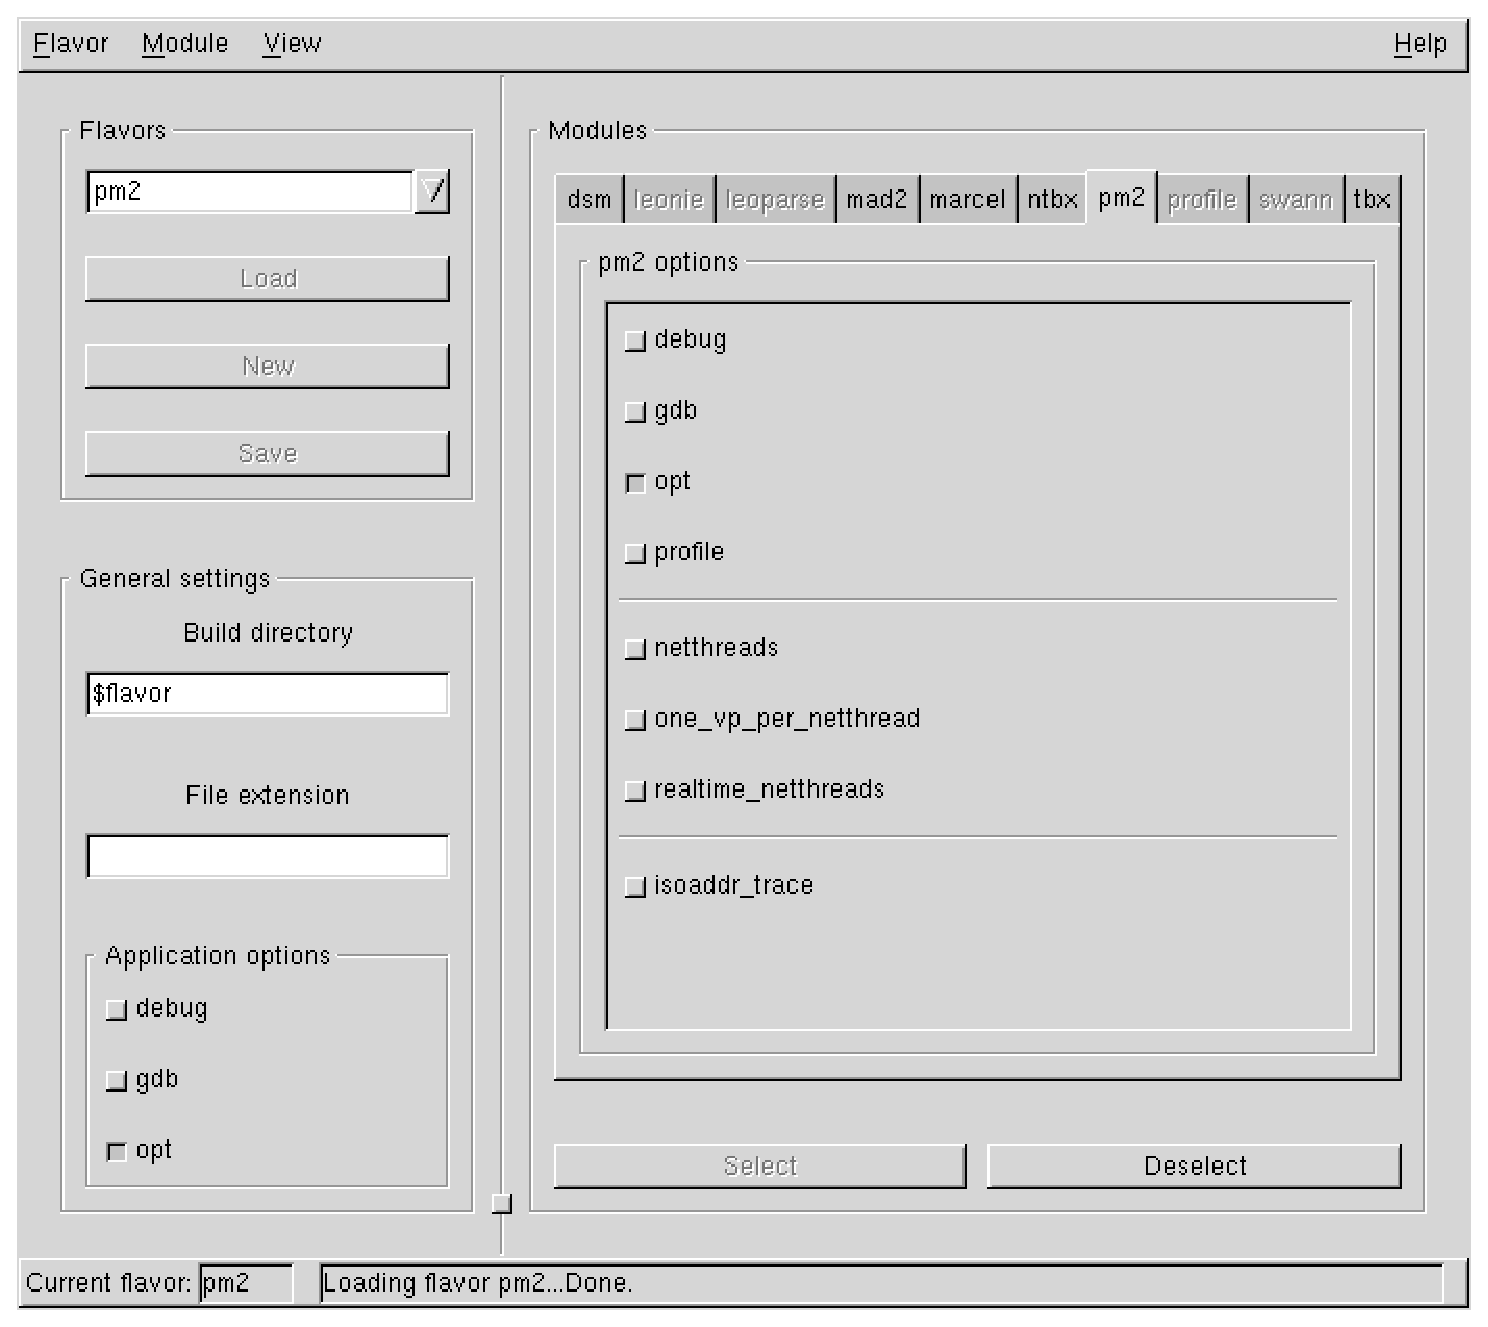
\includegraphics[width=0.7\linewidth]{Figures/ezflavor.eps}
\end{center}
\caption{The \|ezflavor| graphic interface to manage PM2 flavors.}
\label{fig:ezflavor}
\end{figure}

The first step is to analyze your PM2-frustration. 
\begin{shell}
ravel% ezflavor &       # Better run it in background!
\end{shell}
Load in the current flavor \|pm2|.
\begin{itemize}
  
\item Select the \|pm2| module. The result is displayed on
  Figure~\ref{fig:ezflavor}. As you can see, only one option is turned
  on for this module: \|opt|, which makes the module run in optimized
  mode. 
  
\item Select the \|mad3| module: you can observe that the \|tcp|
  option is turned on, which makes Madeleine use the TCP/IP interface.
  
\item Select the \|marcel| module: you can observe the \|mono| option
  is turned on, which makes Marcel run on a single processor at each
  node (even though the node may be have multiple processors). Also,
  you can observe that the \|marcel_main| option is on, which
  specifies that the \|main| function of the C~program is provided by
  PM2 (actually, by Marcel). The user only specifies the auxiliary
  \|pm2_main| function, which is called by the real \|main| function
  after some initialization. See for instance
  program~\ref{prog:hello}.
  
\item Finally, you can observe that the \|opt| option is enabled for
  the application itself: the user code is compiled with the
  \|-O6| option of the \|gcc| compiler.

\end{itemize}

\begin{figure}
\begin{center}
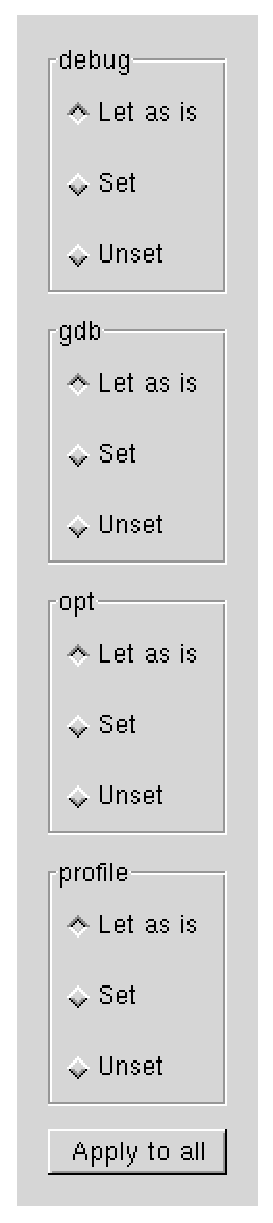
\includegraphics[height=0.4\textheight]{Figures/options.eps}
\end{center}
\caption{The \|Common options| window of the \|ezfalvor| utility.}
\label{fig:options}
\end{figure}

Assume now that the real PM2 you are striving after is a PM2 with
fully-fledged debugging facilities. That's right: what you need is a
\|pm2_debug| flavor, man! 

Check in the \|debug| option in the \|pm2| module.  Do
it for the application, too, and also for the \|mad3| module.
Edit the name of the new flavor from \|pm2| to
\|pm2_debug|, and save it. The new flavor is checked for consistency
and saved under into the \|${PM2_HOME}/.pm2/flavors/pm2_debug|
file. You may check that the file actually contains the modified
flavor:
\begin{shell}
ravel% more ${PM2_HOME}/.pm2/flavors/pm2_debug
# Flavor pm2_debug
[...]
### SETTINGS: --pm2=debug --pm2=opt
[...]
### SETTINGS: --common=debug --common=opt
\end{shell}
Now, you have to recompile PM2 for this new flavor. Observe that you
do not have to explicitly set the \|PM2_FLAVOR| shell variable to
this new value. Just specify it in-line to the \|make| facility.
\begin{shell}
ravel% cd ${PM2_ROOT}
ravel% make PM2_FLAVOR=pm2_debug
[...]           # Well, a bunch of lines here...
\end{shell}
Everything should run smoothly, without any warning...

Once you are done, set the \|PM2_FLAVOR| variable to \|pm2_debug| and
compile your favorite PM2 program using a
``dynamic'' Makefile as the one on Figure~\ref{prog:Makefile1}. Well,
ideally, should you not make any difference with the \|pm2| run. 

Just for fun, modify the \|pm2_debug| flavor so as to enable the
\|isoaddr_trace| in the \|pm2| module, for instance. Recompile PM2
with this modified flavor. Recompile your program, for instance the
simplistic \|hello| on Figure~\ref{prog:hello} and run it. You should
see a lot of rather cryptic debugging information:
\begin{shell}
ravel% pm2-load hello
Alloc page table(6291456)
index 0: 1
index 1: 1
index 2: 1      
[...]
isoaddr_malloc(65536)
isoaddr_malloc: got 16 slots locally
[...]
Hello World!
isoaddr_free: added to stack cache: affe0000 (index = 15)
[Threads : 2 created, 0 imported (0 cached)]
Flushing slot cache...
Flushing stack cache...
Flushing migration cache...
Isoaddr exited
\end{shell}

\begin{warning}
  Be careful that the simple Makefile of Figure~\ref{prog:Makefile1}
  is not able to spot that the flavor has been modified. You will have
  to explicitly delete the object file to create a fresh, consistent
  one. 
\end{warning}

It is often interesting to enable some options for \emph{all} modules
at the same time, together with the application. This holds for the
\|debug|, \|gdb|, \|opt| (optimization) and \|profile| options.
\|ezflavor| provides such a facility: click on the \|View|/\|Common
options| menu to open a specialized window. An example is displayed
on~Figure~\ref{fig:options}.



\paragraph{A note to the wizards.}

Experienced and hurried users may find that the \|ezflavor| interface is
too heavy with respect to their needs. A tty-oriented  interface is
also available. It is called \|pm2-config-flavor|. The default is a 
line-oriented interface:
\begin{shell}
ravel% pm2-config-flavor --text
================= Flavors management ==================
Existing flavors :
default leonie leoparse mad3
marcel marcel_act marcel_actsmp marcel_mono marcel_smp 
pm2 pm2_mad3 pm2_marcel

******************************************************
You can :
 0) create a flavor
 1) modify a flavor
 2) export a flavor
 3) import a flavor
 4) see    a flavor
 5) check  a flavor
 6) remove a flavor
 7) regenerate the flavors
 8) quit this program
\end{shell}

\begin{warning}
  In the current version of the system, no backup copy of a flavor is
  done prior editing. Be careful! 
\end{warning}

\begin{note}
  LB to RN: How should the user could recover the setting of the
  initial \|pm2| flavors, in case of accidental corruption?
\end{note}


\section{Debugging a PM2 program}

You may have already experienced problems in designing PM2 programs.
Debugging distributed, multithreaded programs is a difficult task, and
few tools already exist to assist the programmer in it. One of the
goal of the PM2 project is to contribute to the design of such tools,
but we have rather concentrated on \emph{performance} debugging.
Actually, PM2 is equipped with powerful profiling facilities, to be
introduced in Section~\ref{sec:profiling}. In this section, we rather
concentrate on the tools available at the level of programming.

The first step is to derive a specific flavor from your current one.
It should enable the options \|debug| and \|gdb| for all modules. With
the \|debug| option enabled, the modules of PM2 are careful to check
consistency conditions along the execution, so that abnormal situation
may be detected early. You may also wish to concentrate on memory
allocations by enabling the \|safe_malloc| and the \|parano_malloc|
options of module \|tbx|, the toolbox common to all PM2 modules. If
you suspect a problem with synchronization objects, you will find
useful options in the \|marcel| module.
I you wish to use the \|valgrind| debugger on a program using
\|marcel|, you need to set the \|valgrind| option of the \|marcel|
module to let \|valgrind| know about \|marcel| stacks. If your version
of \|valgrind| is older than 3.0, you will also need to recompile it
after setting, in \|coregrind/vg_memory.c|, the
\|VG_PLAUSIBLE_STACK_SIZE| constant to the size of \|marcel| stacks
(65536 by default).

Assuming that you are using the \|pm2| flavor, make up a
\|pm2_debug| one. Set your \|PM2_FLAVOR| shell variable to this value,
and recompile PM2 with this new flavor. 
\begin{shell}
ravel% setenv PM2_FLAVOR pm2_debug
ravel% cd ${PM2_ROOT}
ravel% make
\end{shell}
Then, recompile the programs of interest with this new flavor. 

\begin{warning}
  Make sure that they are \emph{actually} recompiled: better delete
  the objects files by hand!
\end{warning}


A second step is to insert additional trace outputs within your source
code. Your are strongly advised to print on the \|stderr| error
descriptor instead of regular \|stdout| one. Also, you should always
use the \emph{thread-safe} version of \|(f)printf|, called \|t(f)printf|.
This will prevent multiple Marcel thread to print concurrently,
leading to scrambled text. Use the \|pm2-logs| utility to view the
remote logs. It may be useful to force logging also on the main
node~0: use \|pm2-load -l|. Then, \|pm2-logs| will recover exactly one
log per (logical) node.

You may also require ``immediate'' output from remote node by using
the \|pm2_(f)printf| routine. Each time it is called, the output is
packed into a buffer and sent to main node~0 to be immediately
displayed there. The output is prefixed by \|[t<i>]|, where \|<i>| is
the logical number of the originator node.  This is quite convenient, but
the user has to be aware that the additional messages generated in
this way \emph{do interfere} with the original communication scheme of
the program under debugging. In particular, they may generate
additional deadlocks! Also, these additional messages have to be
considered when designing the termination scheme of the program. The
\|pm2_halt| function should not be called by a node \emph{before} it
is guaranteed that all communications, whatever their origin, have
been handled by the daemon service threads. Deadlock may otherwise
occur.

The \|pm2-load| utility honors a number of options.  The most useful
one in a first place is \|pm2-load -d|. It can be used with any flavor,
but it is most rewarding when the current flavor enables the \|gdb|
for all the modules and for the application. If run with the \|-d|
option, \|pm2-load| opens a \|gdb| session on each (logical) node
declared in the configuration, with a display on your console. Just
typing \|r| (for \|run|) in the window will start the execution.
Observe that your have to type it in \emph{each} window!  Before
debugging your program at this level, you'd better downsize your code
to some manageable configuration, say~3 or 4~nodes. Observe also that
the windows of nodes other than the main one will only pop up after
the main node has started and called its \|pm2_main| routine. Then,
the node is blocked until you have typed \|r| in the window of each
subsidiary node. Before starting the nodes, you may add breakpoints
and require all kind of funcionalities provided by \|gdb|.  PM2 does
not close the windows at the end of the run, so that you can inspect
the final state of each node. Typing \|^D| in each window will close
it and terminate the program.

\begin{warning}
  A note to eye-impaired Solaris users. The \|gdb| facility is run
  within a \|xterm|. In certain recent versions of Solaris, the
  default for the \|xterm| background is a dark grey, which makes
  debugging *very* painful. You can change it to white by adding the
  following line to your \|${HOME}/.Xdefaults| file:
\begin{shell}
xterm*background: White
\end{shell}
Once it is done, reload your \|.Xdefaults| file by issuing:
\begin{shell}
ravel% xrdb -merge < ${HOME}/.Xdefaults
\end{shell}
\end{warning}

The user should be aware that \|gdb| itself is \emph{not} aware
of Marcel threads: \texttt{info threads} will only show LWPs,
\texttt{thread <num>} will only let switch between LWPs, and
\texttt{backtrace} will only show the backtrace of the \emph{current}
Marcel thread running in the chosen LWPs.

However, if Marcel was compiled with the gdb option, Marcel provides
several gdb functions for printing thread state like the --marcel-xtop
option:
\begin{verbatim}
(gdb) marcel-threads
0x3ff4fc00        user_task 43 I  1 machine nil
(gdb) marcel-printthread __main_thread
0xbffefc00             main 43 I  0 machine nil
(gdb)
\end{verbatim}

One may switch to not-running threads' context thanks PM2-provided
functions\footnote{yet implemented on X86 only}:

\begin{verbatim}
(gdb) r
Program received signal SIGINT, Interrupt.
[Switching to Thread 16386 (LWP 25769)]
0x4013c3e7 in sched_yield () from /lib/libc.so.6
(gdb) bt
#0  0x4013c3e7 in sched_yield () from /lib/libc.so.6
#1  0x0804dc6d in idle_func (arg=0x0) at marcel_archdep.h:41
#2  0x0804973a in marcel_create (pid=0x0, attr=0x3ffe0000, func=0, arg=0x0)
    at marcel_sched.h:35
(gdb) set-ctx  __main_thread
switching to __main_thread(0xbffefc40)
(gdb) bt
#0  0x0804d5d8 in marcel_give_hand (blocked=0xbffefb6c)
    at source/marcel_sched.c:1173
#1  0x0804ef40 in marcel_sem_P (s=0xbffefb6c) at source/marcel_sem.c:47
#2  0x08049049 in marcel_main (argc=1, argv=0xbfffcb94) at sumtime.c:75
#3  0x08049dc1 in main (argc=1, argv=0xbfffcb94) at source/marcel.c:1276
(gdb)
\end{verbatim}

One can then use usual functions like \texttt{frame}, \texttt{print},
etc. to inspect the thread.

The user should be aware that although \texttt{set-ctx} achieves a
context switch so as to get correct \texttt{PC} and \texttt{SP},
\texttt{continue}-like commands automatically switch back to the
current running thread\footnote{In theory, the PM2 process should
then continue properly, but it seems gdb does not yet let this work
correctly}.

The user should be aware that some of the names of PM2 routine are in
fact on-line definitions in internal header files. Thus, one has to
know the \emph{actual} name of the routine to set a breakpoint. The
following table provides the some useful translations.
\begin{center}
\begin{tabular}{|l|l|l|}
\hline
External name & Real name & Origin module \\
\hline
\|pm2_init|     & \|common_init|        & \|pm2| \\
\|pm2_main|     & \|marcel_main|        & \|pm2| \\
\hline
\|tprintf|      & \|marcel_printf|      & \|tbx| \\
\|tfprintf|     & \|marcel_fprintf|     & \|tbx| \\
\hline
\|lock_task|    & \|ma_lock_task|       & \|marcel| \\
\|unlock_task|  & \|ma_unlock_task|     & \|marcel| \\
\hline
\end{tabular}
\end{center}


